
\chapter{状态等价最小化}
本节中,我们限定在完全$DFA$的最小化中。\uline{This is strictly a notational convenience, as the minimization algorithm can be modified to work for non-complete DFA.严格地说,这是一种标记的便利,因为可以对最小化算法进行修改,使其适用于不完全DFA。} 除非$DFA$的语言是$V^*$,否则完全最小化$DFA$比不完全最小化DFA多一个状态(sink)。令 $ M = (Q,V,T,\theta,S,F)$ 为完全$DFA$,这个特殊的$DFA$将会贯穿本节内容。我们也假设所有的 $M$ 的所有状态都是从开始状态可以到达的,也就是$Useful_s(M)$。由于 $M$ 是确定且完全的,我们也把转移关系 $T \in Q \times V \longrightarrow Q$ 称为全函数,而不是 $T \in Q \times V \longrightarrow \mathcal{P}(Q)$。

为了最小化 $DFA$ $M$,我们计算等价关系 $E \subseteq Q \times Q$,将其定义为\\
$\mbox{   } (p,q) \in E \equiv ( \overrightarrow{\mathcal{L}}(p) = \overrightarrow{\mathcal{L}}(q) )$ \\
\uline{Since this is an equivalence relation, we are really interested in unordered pairs of states. 由于这是一个等价关系,我们确实对无序状态对有兴趣},使用有序对比使用无序对更方便。

根据等价关系 $E$ ,使用 \textit{merge} 转换来对等价关系进行合并。
\newline

\noindent{\textbf{转换 3.1 (合并状态)} : 对于任何满足 $ H \in E $ 的等价关系 $H$, 函数 $merge$ 可以用来减少 ${DFA}$的状态数\footnote{当$H$是状态上的恒等关系时,函数$merge$不会减少状态的数量。} ,函数 $merge$ 定义为:}

\begin{displaymath}
    \begin{split}
    & merge((Q,V,T,\emptyset,\{s\},F),H)  = \mbox{\textbf{let} }  T' = \{([p]_H,a,[q]_H):(p,a,q)\in T\} \\
    & \mbox{              \textbf{in}}\\
    & \mbox{                 } ([Q]_H,V,T',\emptyset,\{[s]_H\},[F]_H) \\
    & \mbox{              \textbf{end}}
    \end{split}
\end{displaymath}

% 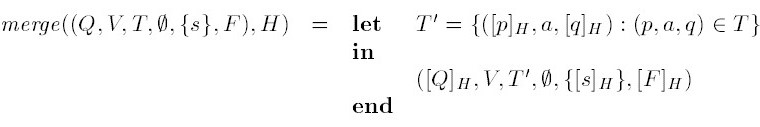
\includegraphics[width =.9\textwidth]{figure2.jpg}

$merge$ 的定义独立于等价类的代表的选择。函数 $merge$ 拥有以下性质:
\begin{equation*}
    \mathcal{L}_{FA}(merge(M,H)) = \mathcal{L}_{FA}(M) \land | merge(M,H) | \leq |M| \land | merge(M,H)| = \sharp H
\end{equation*}
它保留了 $Complete$, $\epsilon$-$free$, $Useful$, $Det$, 和 $minimal$ 等性质; 当然, $merge$ 仅定义在 $\epsilon$-$free$ 和 $DFA$ 上。

为了计算关系$E$, 需要函数$\overrightarrow{\mathcal{L}}$的一个性质。
\newline

\noindent{\textbf{性质3.2 (函数$\overrightarrow{\mathcal{L}}$)}: 函数$\overrightarrow{\mathcal{L}}$ 满足 }
$$ \overrightarrow{\mathcal{L}}(p) = (\cup a:a \in V : \{a\} \cdot \overrightarrow{\mathcal{L}}(T(p,a))) \cup ( \mbox{ \textbf{if} }   (p \in E) \mbox{ \textbf{then} }   \{\epsilon\} \mbox{ \textbf{else} }   {\emptyset  \mbox{ \textbf{fi} }}) $$
\uline{This allow us to give an alternate characterization of equivalence of states. 这允许我们给出状态等价的另一种描述}。  
\newline

\noindent{\textbf{定义 3.3 (状态的等价):} \uline{等价关系 $E$ 是最大不动点}(在细化的情况下): } \\
$\mbox{  } (p,q) = E \equiv ( p \in F \equiv q \in F ) \land ( \forall a:a \in V : (T(p,a),T(q,a)) \in E )$
\newline
\\
\noindent{\textbf{备注3.4:} \uline{the greatest fixed point has the least number of equivalence classes of any such fixed point. 最大不动点拥有最少的任何此类不动点的等价类数。} }
\newline

\noindent{\textbf{备注3.5:} 定义3.3中的任何不动点都可以使用。为了最小化自动机,需要最大不动点。}
\newline

\noindent{\textbf{性质3.6(近似$E$)}: 我们可以用连续逼近来计算最大不动点,E的连续逼近如下($ k \ge 0 $ ):} \\
\mbox{   }$(p,q) \in (E_{k+1} \equiv (p,q) \in E_k \land (\forall a:a \in V : (T(p,a),T(q,a))\in E_k ) $ \\
$E_0$ 定义为:\\
\mbox{   }$(p,q) \in E_0 \equiv (p \in F \equiv q \in F)  $ \\
$E_0$ 的一个等价定义是 $E_0 = (Q \setminus F)^2 \cup F^2$。 对于所有的 $K \ge 0$ 有 $E_{k+1} \in E_k$。
\newline

\noindent{\textbf{备注3.7}: 如果$E_k$是一个等价关系,那么$E_{k+1}$也是。$E_0$是一个等价关系。}
\newline

\noindent{\textbf{备注3.8}: 有一个直观的 $E_k$ 的说明是有用的。\uline{当且仅当没有字符串 $ w: |w| \leq k $ 满足 $ w \in \overrightarrow{\mathcal{L}}(p) \not\equiv w \in \overrightarrow{\mathcal{L}}(q) $一个状态对 $p,q$ 也可以说成 $k$-等价 (写作 $(p,q)\in E_k$) }。作为结果,当且仅当 }

\begin{itemize}
    \item [-] 两者都是最终态或者都不是最终态;
    \item [-] 所有的 $a\in V,T(p,a) \mbox{和} T(q,a)$ 都是 ($k$-1)-等价(根据 $\overrightarrow{\mathcal{L}}$ 和 $T^*$ 的定义  );
\end{itemize}
时 $p$ 和 $q$ 都是 $k$-等价。
\newline

\noindent{\textbf{备注3.9}: E的一个重要性质是,它也是包含于(set containment instead of refinement)定义3.3中等价性的最大的固定点。作为最大的不动点,E可以用$\subseteq$-descending 关系序列来计算,从 $Q\times Q$ 开始,这样的序列不必只包含等价关系。在这样的近似序列中可能有比在上面给出的$E_k$序列有更多的步骤。幸运的是,每个这样的步骤通常都比从$E_k$计算$E_{k+1}$更容易计算。较容易计算这些(但较长)序列的一些算法在第4.2-4.5和第4.7节中给出。}

所有先前已知的算法都是通过上面的连续逼近法(相对于 $\subseteq$)计算E。\uline{第4.7节中的新算法通过以下逐次逼近来计算 $E$ }。在这一节中,解释了这一点的实际重要性。



%%%%%%%%%%%%%%%%%%%%%%%%%%%%%%%%%%%%%%%%%%%%%%%%%%%%%%%%%%%%%%%%%%%%%%%%%%%%%%%%%%%%%%%%%%%%%%%%%%%%%%%%%%%%%%%%%%
\section{可区分性}
通过先计算 $E$ 的补集 $D=\neg E$ 来计算 $E$ 是有可能的。关系 $D$ (也叫做状态关系的可区分性)定义为 \\
\mbox{   }$ (p,q) \in D \equiv (\overrightarrow{\mathcal{L}}(p) \not=\overrightarrow{\mathcal{L}}(q)) $\\
%\newline

\noindent{\textbf{定义3.10(状态的可区分性)}:$D$ 是一个方程中的最小(under $\subseteq$, set containment\footnote{这里,$\subseteq$代表设置标准容量;因为$D$不一定是等价关系,所以refinnement并不适用。})不动点} \\
\mbox{   }$ (p,q)\in D \equiv (p \in F \not\equiv q \in F) \land (\exists a:a \in V : (T(p,a)) \in D) $\\
%\newline

\noindent{\textbf{性质3.11 (逼近D)}: 随等价关系E,关系D可以通过连续逼近来计算 ($k\ge 0$)}
$$ (p,q) \in D_{k+1} \equiv (p,q) \in D_k \land ( \exists a:a \in V : (T (p,a),T(q,a))\in D_k)$$
有 $D_0 = \neg E_0 = ( (Q \setminus F) \times F) \cup ( F \times ( Q \setminus F))$, 对于所有的 $k \ge 0$ ,有 $D_k = \neg E_k$, 同时 $D_{k+1} \subseteq D_k $。
\newline

\noindent{\textbf{备注3.12}: 对于 $E_k$,有一个直观的 $D_k$ 的说明是有用的。\uline{当且仅当没有字符串 $ w: |w| \leq k $ 满足 $ w \in \overrightarrow{\mathcal{L}}(p) \not\equiv w \in \overrightarrow{\mathcal{L}}(q) $一个状态对 $p,q$ 也可以说成 $k$-$distinguished$ (写作 $(p,q)\in E_k$) }。作为结果,当且仅当}

\begin{itemize}
    \item [-] 其中一个是最终态而另外一个不是最终态;
    \item [-] 存在 $a\in V$ such that $T(p,a)$ 和 $T(q,a)$ 是 在 $(k-1)$-$distinguished$。
\end{itemize}
时 $p$ 和 $q$ 是 k-distinguished (一些作者也把它叫做 $k$-$distinguishable$)。



\section{近似步骤数的上界}
我们可以很容易的把一个近似步骤数的上界放进$E$的计算当中。

设$E_j$为定义$E$的方程的最大不动点,可以得到以下逼近步骤(where $I_Q$ 是状态上的恒等关系):
$$ E_0 \subset E_1 \subset \cdots \subset E_j \in I_Q $$
近似序列中部分等价关系的指数是已知的:$\sharp I_Q = |Q| \mbox{且} \sharp E_0 \leq 2$,可以推导出:
$$ \sharp E_0 < \sharp E_1 < \cdots < \sharp E_j \leq \sharp I_Q = |Q| $$
$\sharp E_0=0$时,$E_0$是最大不动点。$\sharp E_1=1$时,要么所有状态都是终态,要么所有状态都不是终态。两种情况下$E_0$都是最大不动点。$\sharp E_0=2$时,$i+2 \leq \sharp E_i$,由 $ j+2 \leq \sharp E_j \leq \sharp I_Q = |Q| $ 可得 $j \leq |Q|-2 $ 。这给出了计算(从$E_0$开始)最大不动点$E_j$的步骤$(|Q|-2)$ 的上界,最大值0(使用性质3.6中的逼近序列)。

上界为$E=E_{(|Q|-2)\textbf{max} 0}$。正如之后我们会见到的那样,它可以为算法带来效率上的提升。这个结果同样在 Wood \cite[引理  2.4.1]{Wood87} 中有所记录。This upperbound also holds for computing $D$ and $[Q]_E$ by approximation。


\section{描述$E$的等价类}

计算$[Q]_E$: $E$的等价类集合 同样是可行的。为了分割 $[Q]_E$,我们由定义3.3出发,把$E$的等价类描述为最大等价关系:
\begin{equation*}
    \begin{split}
        & \mbox{  }(\forall p,q : (p,q) \in E : ( p \in F \equiv q \in F ) \land ( \forall a:a \in V : (T(p,a),T(q,a)) \in E )) \\
        & \equiv \mbox{\{ definition of membership in E; more a to outer quantification \} }\\
        & \mbox{  }(\forall p,q,a:(p,q)\in E \land a\in V : (p \in F \equiv q \in F) \land [T(p,a)]_E = [T(q,a)_E]) \\
        & \equiv \mbox{\{ Introduce equivalence classes } Q_0,Q_1\mbox{ explicity\} } \\
        & \mbox{  }(\forall Q_0,Q_1,a:Q_0\in [Q]_E \land Q_1 \in [Q]_E \land a \in V : \\
        & \mbox{  }(\forall p,q:p\in Q_0 \land q\in Q_0 : (p \in F \equiv q \in F) \land T(p,a) \in Q_1 \equiv T(q,a) \in Q_1))
    \end{split}
\end{equation*}
\newline

\noindent{\textbf{定义 3.13(函数 $Splittable$)}: 为了使其更简洁,我们定义}
$$ Splittable(Q_0,Q_1,a) \equiv (\exists p,q:p\in Q_0 \land q\in Q_0 : (T(p,a) \in Q_1 \not\equiv T(q,a) \in Q_1)) $$
使用$Splittable,[Q]_E$ 最大的划分 (在 $\sqsubseteq$ 的情况下),那么 $[Q]_E \sqsubseteq [Q]_{E_0}$,且有
$$ (\forall Q_0,Q_1,a:Q_0 \in [Q]_E \land Q_1 \in [Q]_E \land a \in V : \neg Splittable(Q_0,Q_1,a)) $$
可以用在$[Q]_E$的计算中。